При обзоре литературы были изучены различные подходы к решению задачи подбора оптимальной конфигурации микроархитектуры процессора. В начале приводится теоретическое описание задачи, а также выводится полезная формула для оценки времени работы алгоритма, на основании которой в дальнейшем происходит классификация методов решения задачи подбора оптимальных параметров на два типа.


\section{Теоретическая основа}\label{sec:theor_base}

Задача подбора оптимальной конфигурации микроархитектуры процессора сводится к задаче максимизации функции нескольких переменных в некой области многомерного пространства. В рассматриваемой задаче в качестве максимизируемой функции будет выступать среднее число инструкций исполненных за один такт~--- Instructions per cycle (далее~--- IPC) по определению равное
\begin{equation}\label{eq:IPC}
  \text{IPC} = \dfrac{\text{число исполненных инструкций}}{\text{число прошедших тактов процессора}}.
\end{equation}
Откуда нетрудно заметить, что $\text{IPC} > 0$ (неотрицательность IPC очевидна, а неравенство IPC нулю следует из того, что в данной задаче интересно рассмотрение только <<реальных>> трасс исполнения, содержащих ненулевое число инструкций). В некоторых работах вместо IPC используется среднее число тактов потраченное на одну инструкцию~--- Cycles per instruction (далее~--- CPI), которое определяется как
\begin{equation}\label{eq:CPI}
  \text{CPI} = \dfrac{\text{число прошедших тактов процессора}}{\text{число исполненных инструкций}} = \dfrac{1}{\text{IPC}}.
\end{equation}

В данной задаче IPC рассматривается как функция:
\[
  \text{IPC} = f\left(x_1, x_2, \dots, x_n\right).
\]
При этом параметры микроархитектуры процессора (далее для простоты изложения могут называться просто параметрами) со значениями $x_1,x_2,\dots,x_n$, вообще говоря, могут иметь зависимости между собой, обусловленные естественными законами (как например, зависимость числа промахов в кэше от его размера при прочих равных условиях), дополнительными ограничениями на процессор, его стоимостью (нельзя увеличивать все параметры бесконечно), а также иными причинами.

Исходя из вышесказанного, задача формулируется следующим образом:
\[
  \begin{cases}
    \hfil\text{IPC} = f\left(x_1, x_2, \dots, x_n\right) \\
    \hfil G =
    \left\lbrace
    \vec{x} \in \mathbb{R}^n | \, a_i \leqslant x_i \leqslant b_i, \,
    i = \overline{1 \dots n}
    \right\rbrace \\
    \hfil f: G \rightarrow \mathbb{R}^{ + } & \text{(из \formref{eq:IPC})}
  \end{cases}
\]
С дополнительными условиями:
\begin{equation}\label{eq:ipc_add}
  \system{
    \phi_i : G \rightarrow \mathbb{R}, \, i = \overline{1\dots n} \\
    \displaystyle\sum_{i = 1}^{m} \left(
    \phi_i \left(
    x_1, x_2, \dots, x_n
    \right)
    \right)^2 \equiv 0
  },
\end{equation}
где $G$ называется \textbf{пространством конфигураций} или \textbf{конфигурационным пространством}.
Требуется найти (при соблюдении условий \formref{eq:ipc_add})
\[
  \text{IPC}_{optimal} = \max_{\lvec{\left(x_1, x_2, \dots, x_n\right)} \in G} f\left(x_1, x_2, \dots, x_n\right)
\]
Либо же если задано пороговое значение IPC:
\[
  \text{IPC}_{optimal} = f\left(x_1^{optimal}, x_2^{optimal}, \dots, x_n^{optimal}\right) \geqslant \text{IPC}_{threshold}
\]
Тогда найденные параметры $x_1^{optimal},x_2^{optimal},\dots,x_n^{optimal}$ задают оптимальную конфигурацию процессора.

Данную задачу можно проиллюстрировать следующей схемой (для случая $\mathbb{R}^3$):
\begin{figure}[!ht]
  \centering
  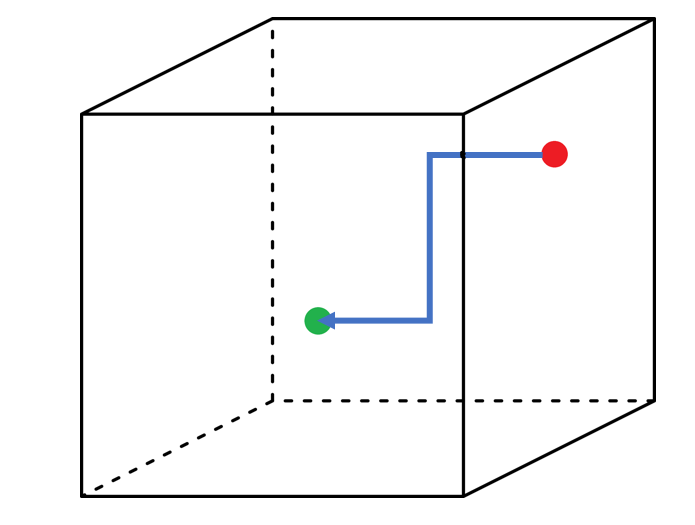
\includegraphics[width=0.6\linewidth]{cube.png}
  \caption{Схема работы алгоритма подбора параметров}
  \label{fig:cube}
\end{figure}

На схеме, изображённой на \picref{fig:cube}, куб изображает пространство конфигураций, красная точка~--- начальную точку, отвечающей начальной конфигурации процессора, зелёная точка~--- желаемую точку, в которой достигается максимальное (либо требуемое) IPC.

Рассмотрим пространство конфигураций более подробно. Обычно параметры микроархитектуры процессора могут принимать лишь дискретный набор значений, следовательно число точек в пространстве конфигураций конечно и может быть вычислено по правилу умножения~\cite[25]{окулов2014дискретная}:
\begin{equation}\label{eq:NG}
  N_G = \prod_{i = 1}^{n} \left|p_i\right|,
\end{equation}
где $p_i$~--- множество значений параметра с индексом $i$, $\left|p_i\right|$~--- его мощность (количество значений параметра с индексом $i$), при этом очевидно, что $\forall i \,\,\, x_i \in p_i$.

Пусть $\Delta t$~--- время однократного исполнения трассы на симуляторе, $N$~--- число точек конфигурационного пространства, в которых требуется исполнить трассу. Тогда полное время исполнения одной трассы на симуляторе в $N$ точках пространства конфигураций вычисляется по очевидной формуле:
\begin{equation}\label{eq:TN}
  T_N = N \cdot \Delta t.
\end{equation}

Используя формулы \formref{eq:NG} и \formref{eq:TN}, можно оценить время, требуемое для исполнения одной трассы во всех точках пространства конфигураций (метод полного перебора):
\begin{equation}\label{eq:bf_time}
  T_{G} = N_G \cdot \Delta t = \prod_{i = 1}^{n} \left|p_i\right| \cdot \Delta t.
\end{equation}

Решение методом полного перебора, очевидно, способно найти точку конфигурационного пространства с наибольшим IPC, однако из-за огромного числа параметров современного процессора, а также длительного времени симуляции на моделях производительности, время $T_G$ из \formref{eq:bf_time} становится значительно больше разумных сроков для решения данной задачи. В этой связи разрабатываются подходы, уменьшающие время работы симулятора для нахождения оптимальной конфигурации процессора. Исходя из формулы \formref{eq:TN}, можно разделить потенциальные методы решения задачи поиска оптимальной конфигурации микроархитектуры процессора на два класса:
\begin{itemize}
  \item решения, уменьшающие $\Delta t$~--- методы ускорения симуляции
  \item решения, уменьшающие $N$~--- методы ускорения непосредственно алгоритма подбора через уменьшение числа точек пространства конфигураций, в которых требуется запустить симулятор
\end{itemize}

Перейдём к рассмотрению существующих методов\,--\,представителей вышеперечисленных классов.

\section{Решения, уменьшающие время симуляции}

Данный класс решений фокусируется на ускорении работы симулятора. Методы данного класса предлагают использовать аппаратные решения~\cite{chiou2007fpga}, а также ряд оптимизаций на программном уровне~\cite{miller2010graphite,carlson2011sniper}.

Нетрудно заметить, что  с увеличением числа параметров и количества их значений число симуляций $N_G$ сильно растёт, и ускорение, получаемое методами данного класса, нивелируется, не оказывая заметного влияния на возрастание $T_G$.

\section{Решения, ускоряющие алгоритм подбора}

\subsection{CPI stack подходы}

В данных подходах используется метод CPI stack, в основе которого лежит идея о разложении среднего числа тактов, потраченных на одну исполненную инструкцию~--- CPI~\formref{eq:CPI} на независимые слагаемые. Обычно выделяют базовую (обязательную), а также некоторый набор компонент, отражающих такты, <<потерянные>> из-за таких событий как ошибки предсказания переходов, промахи в кэшах и буферах ассоциативной трансляции (англ.~TLB) и т.~д.~\cite{eyerman2006performance}:
\begin{align}\label{eq:CPIstack}
  \begin{split}
    \text{CPI} &= \dfrac{
      \text{обязательные такты} + \text{такты на кэш} + \text{такты на TLB} + \dots
      }{\text{число исполненных инструкций}}\\
      &= \frac{\text{обяз. такты}}{\text{число исп. инструкций}} + \frac{\text{такты кэш}}{\text{число исп. инструкций}} + \dots\\
      &= \text{CPI}_{\text{обяз}} + \text{CPI}_{\text{кэш}} + \text{CPI}_{\text{TLB}} + \dots
  \end{split}
\end{align}

При аккуратном подсчёте, CPI stack позволяет указать на узкие места в конфигурации процессора, сужая множество параметров\,--\,кандидатов на изменение. Например, в~\cite{lee2014rpstacks} рассматривается использование CPI stack полученного с помощью анализа критического пути в конвейере процессора. Такой подход позволяет более точно оценить причины потери циклов процессора, однако анализ критического пути является затратной (а также сложной в реализации) операцией, значительно увеличивающей время симуляции. Именно поэтому в~\cite{eyerman2017multi} предлагается вместо усложнения алгоритма вычисления CPI stack, вычислять сразу несколько CPI stack на разных стадиях конвейера процессора. Данное представление даёт более полную картину о событиях, влияющих на производительность процессора, а также диапазон ожидаемых улучшений производительности процессора в случае ликвидации конкретного события простоя.


\subsection{Подходы с использованием машинного обучения}


Исходя из теоретического описания задачи, представленного в разделе~\ref{sec:theor_base}, можно заключить, что рассматриваемая задача сводится к задаче оптимизации, для решения которой можно использовать методы машинного обучения.

Подходы с использованием машинного обучения~\cite{joseph2006construction,ipek2006efficiently,chen2014archranker} предлагают использовать модели, обученные на некотором относительно небольшом подмножестве пространства конфигураций, для предсказания IPC во всех остальных точках пространства.
Например, в~\cite{joseph2006construction} предлагается решать задачу подбора параметров как задачу линейной регрессии:
% \[
  \begin{multline}
    y = \beta_0 + \sum_{i = 1}^{m} \beta_i x_i + \sum_{i = 1}^{m}\sum_{j = i + 1}^{m}\beta_{i,j}x_ix_j \\  +\sum_{i = 1}^{m}\sum_{j = i + 1}^{m}\sum_{k = j + 1}^{m} \beta_{i,j,k} x_ix_jx_k
    \dots \\  +\beta_{1,2,\dots,m}x_1x_2\dots x_m,
  \end{multline}
% \]
где в качестве выходного параметра $y$ выступает CPI (дополнительно проводится исследование с целью выбрать функцию от IPC в качестве выходного параметра, которая обладает наименьшей ошибкой), а подбираемые коэффициенты $\beta$ играют роль важности соответствующего параметра. В работе также указывается, что для хорошей сходимости и высокой точности решения обычно достаточно не слишком большое множество параметров микроархитектуры процессора~--- достаточно лишь выделить некое подмножество.

В~\cite{ipek2006efficiently} применяется более сложный подход с использованием моделей нейронных сетей. В работе предлагается модель, которой достаточно обучится на 1\% от всего пространства конфигураций, для того чтобы выдавать высокоточные предсказания. Перед передачей параметров процессора нейронной сети, производится их нормировка в интервал $(0,1)$ c помощью min max scaling~\cite[114]{han2012data}, включая категориальные параметры (для них используется метод one-hot encoding~\cite{brownlee2017one}). Далее происходит тренировка некого набора нейронных сетей с применением перекрёстной валидации~\cite{stone1978cross}. Также стоит отметить, что каждая точка конфигурационного пространства из тренировочного набора подается сетям с частотой, пропорциональной CPI в этой точке.

В противовес предыдущему решению, в~\cite{chen2014archranker} описывается несколько иной подход с использованием машинного обучения, решая вместо классической задачи нахождения экстремального значения, задачу классификации. Данная задача состоит в том, чтобы выделить из двух предоставленных конфигураций микроархитектуры процессора <<лучшую>>. Такие попарные сравнения позволяют без дополнительных расходов на симуляцию увеличить размер тренировочного множества с $n$ до $\frac{n\cdot \left(n - 1 \right)}{2} = \mathcal{O}\left(n^2\right)$, что существенно улучшает точность предсказания.

В~\cite{dubach2010empirical} сообщается о двух недостатках, которыми обладают некоторые вышеописанные модели:
\begin{itemize}
  \item При смене тестовых наборов требуется заново собирать и обучать модель
  \item Для обучения существующих предсказателей обычно требуется большое число симуляций
\end{itemize}
Предлагаемая модель фокусируется на поведении самой микроархитектуры. В основе метода лежит идея о разложении нового пространства, представляющего новую программу на на линейную комбинацию пространств тестовых программ, где в роли метрики выступает производительность.
\begin{figure}[!ht]
  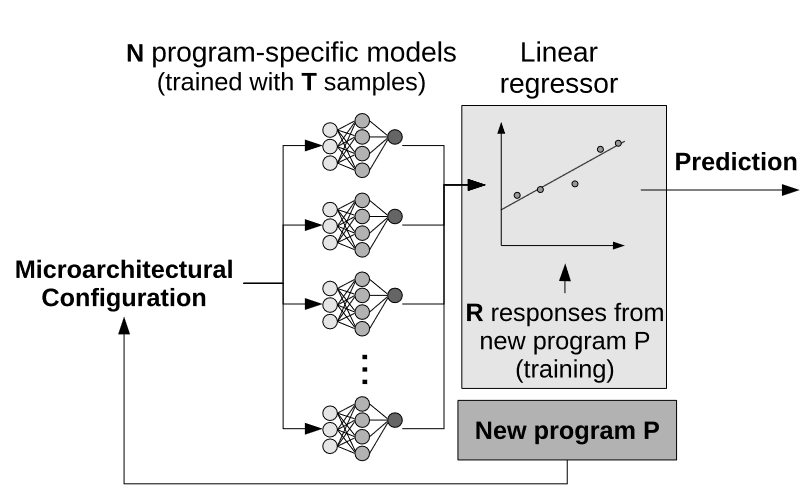
\includegraphics[width=\linewidth]{ML.png}
  \caption{Схема алгоритма~\cite{dubach2010empirical}}
  \label{fig:empirical}
\end{figure}
На \picref{fig:empirical} изображена схема предлагаемого решения. Решение работает следующим образом. Сначала происходит обучение $N$ моделей, каждая на своём приложении, далее при для предсказания  поведения новой программы, собирается результат малого числа $R$ симуляций новой программы, а также результаты предсказаний моделей с этих симуляций, после чего используется метод линейной регрессии в следующем виде:
\[
  \lvec{y} = \beta_0 + \sum_{i = 1}^{m} \beta_i \cdot \lvec{X}_i,
\]
где $\lvec{X}_j$~--- вектор из $R$ ответов от модели $j$, $\lvec{y}$~--- вектор, состоящий из ответов новой программы на $R$ симуляциях. Таким образом, для получения предсказания для новой программы на очередной точке конфигурационного пространства, достаточно подать $R$ новых точек пространства на обученные предсказатели (модели), получая тем самым нужные $R$ ответов.

Перечисленные методы позволяют значительно сократить число симуляций $N$.

\section{Анализ решений}

В существующих работах, как правило, рассматривается варьирование параметров высокого порядка\footnote{Параметры, небольшое изменение которых приводит к значительному изменению производительности}, такие как размер кэша, алгоритм предсказания условных переходов и т.~п. В то время как наибольшую сложность на практике представляет варьирование параметров низкого порядка (дополнительный бит в алгоритме предсказания, дополнительный бит тэга).

С одной стороны, исходя из определения, изменение одного параметра микроархитектуры низкого порядка не может привести к такому значительному изменению производительности процессора, как при изменении одного параметра микроархитектуры высокого порядка. С другой стороны, при одновременном изменении нескольких параметров микроархитектуры низкого порядка, можно добиться существенного прироста производительности процессора.

Существующие решения не позволяют эффективно находить оптимальные конфигурации микроархитектуры процессора при рассмотрении большого числа параметров низкого порядка:
\begin{itemize}
  \item Подходы основанные на RpStacks имеют высокую сложность реализации, в силу того, что стандартные данные о задержках, предоставляемые разработчиками симуляторов, не покрывают эффективно параметры микроархитектуры низкого порядка.
  \item Эмпирические модели машинного обучения, которые предлагается использовать для предсказания производительности процессора, из-за нетривиального характера взаимного влияния параметров низкого порядка требуют намного больше данных для обучения, что выражается в большем числе запуска симулятора, отрицательно сказываясь на времени работы
\end{itemize}
